\documentclass[11pt,letterpaper]{article}
\usepackage[margin=0.86in]{geometry}
\usepackage[T1]{fontenc}
\usepackage[utf8]{inputenc}
\usepackage{lmodern}
\usepackage{xcolor}
\usepackage{graphicx}
\usepackage{tabularx,booktabs,array,longtable}
\usepackage{enumitem}
\usepackage{hyperref}
\usepackage{fancyhdr}
\usepackage{lastpage}
\usepackage{titlesec}
\usepackage{amsmath,amssymb}
\usepackage{microtype}
\usepackage{needspace}
\usepackage{ragged2e}
\definecolor{navy}{HTML}{19334C}
\definecolor{teal}{HTML}{236B82}
\definecolor{soft}{HTML}{EFF5F7}
\definecolor{muted}{HTML}{52616B}
\hypersetup{colorlinks=true,linkcolor=teal,urlcolor=teal}
\titleformat{\section}{\Large\bfseries\color{navy}}{\thesection.}{0.6em}{}
\titleformat{\subsection}{\large\bfseries\color{navy}}{\thesubsection}{0.6em}{}
\titleformat{\subsubsection}{\normalsize\bfseries\color{navy}}{\thesubsubsection}{0.6em}{}
\titlespacing*{\section}{0pt}{15pt}{6pt}
\titlespacing*{\subsection}{0pt}{10pt}{4pt}
\setlength{\parindent}{0pt}
\setlength{\parskip}{4.5pt}
\setlength{\headheight}{15pt}
\renewcommand{\arraystretch}{1.16}
\setlist[itemize]{topsep=3pt,itemsep=2pt,leftmargin=1.4em}
\setlist[enumerate]{topsep=3pt,itemsep=2pt,leftmargin=1.5em}
\pagestyle{fancy}
\fancyhf{}
\fancyhead[L]{\small\color{muted} Applied Machine Learning \textbar{} Cornell Tech}
\fancyhead[R]{\small\color{muted} Human or AI?}
\fancyfoot[C]{\small\color{muted} Page \thepage\ of \pageref{LastPage}}
\renewcommand{\headrulewidth}{0.3pt}
\newcommand{\placeholder}[1]{\par\noindent\textcolor{teal}{\textit{[Your response: #1]}}\par\vspace{0.3em}}
\newcommand{\figplaceholder}[1]{\par\noindent\fcolorbox{teal}{soft}{\parbox[c][1.15in][c]{0.94\linewidth}{\centering\textcolor{muted}{Insert #1 here}}}\par}
\newcommand{\question}[2]{\needspace{4\baselineskip}\par\addvspace{0.45em}\noindent\textbf{#1}\quad #2\par\nobreak\vspace{0.1em}}
\newcommand{\smallnote}[1]{{\small\color{muted}#1}}
\newcolumntype{Y}{>{\RaggedRight\arraybackslash}X}
\begin{document}
\thispagestyle{empty}
\vspace*{0.2in}
{\color{teal}\bfseries CORNELL TECH \textbar{} APPLIED MACHINE LEARNING}\par
\vspace{0.15in}
{\Huge\bfseries\color{navy} Human or AI?}\par
\vspace{0.07in}
{\LARGE\color{navy} Kaggle Competition \&  Report Template}\par
\vspace{0.17in}

\textbf{Report Template: }\href{https://www.overleaf.com/project/6ae1fc85355dcf680137d898/share#f2777b20d3adeeecfac9096f78008e2f8daa0ff4be43de3b}{TEMPLATE}

\textbf{Github Repository Template: }\href{https://github.com/sekhari/human-or-ai-submissions}{REPO}

\textbf{Welcome to the competition!} Your task is to build a machine learning classifier that predicts whether a passage was written by a human or generated by an AI model. You will use a labeled training set, an additional unlabeled set, and a held-out Kaggle test set. The aim is not just a high leaderboard score: we want you to compare methods, design careful experiments, understand generalization, and explain what your results actually show.

You are encouraged to try several approaches. A well-tested logistic regression or support vector machine is just as legitimate as a neural network. The project is designed to be approachable on a laptop; a GPU is \emph{not required} for full credit.

\vspace{0.06in}
\begin{tabularx}{\linewidth}{@{}>{\bfseries}p{1.58in}Y@{}}
Team / members & Zhitong Liu (zl2358); Sorathorn Thongpitukthavorn (st2329); Keyan Miao (km2299) \\
Kaggle team name & team 35 \\
GitHub PR URL & \href{https://github.com/sekhari/human-or-ai-submissions/pull/6}{https://github.com/sekhari/human-or-ai-submissions/pull/6} \\
\end{tabularx}
\vspace{0.06in}
\subsection*{Your data}
\begin{tabularx}{\linewidth}{@{}lrrY@{}}
\toprule
\textbf{File} & \textbf{Rows} & \textbf{Labels} & \textbf{Purpose} \\
\midrule
\texttt{train.csv} & 10,000 & Visible & Supervised model development: 5,000 human (0), 5,000 AI (1) \\
\texttt{unlabeled.csv} & 3,000 & Hidden & Optional input for semi-supervised methods; required experiment \\
\texttt{test.csv} & 3,000 & Hidden & Predict the probability of AI authorship for Kaggle \\
\texttt{train\_starter\_2000.csv} & 2,000 & Visible & Convenient subset of \texttt{train.csv} for quick experiments \\
\bottomrule
\end{tabularx}

\smallnote{The starter data is a subset, not 2,000 additional labeled examples. Passages are approximately 75--350 words, with mean length near 210 words.}

\subsection*{How the test set works}
The test set mixes familiar and unfamiliar writing domains and AI generators, and includes some adversarially modified AI-written passages. You will \emph{not} receive labels, source model names, domain labels, or difficulty memberships for individual test examples. Submit a probability in $[0,1]$ for each test ID, where 1 means AI-generated. Kaggle evaluates submissions using \textbf{area under the ROC curve (AUROC)}. The \textbf{public leaderboard} covers 900 examples (30\%); the \textbf{private leaderboard} covers 2,100 (70\%) and determines the final competition performance score.


\vfill
\newpage
\section{Competition rubric and submission instructions}
\begin{tabularx}{\linewidth}{@{}Y>{\raggedleft\arraybackslash}p{0.85in}@{}}
\toprule \textbf{Component} & \textbf{Points}\\ \midrule
Kaggle private leaderboard performance & 25 \\
Model comparison and selection & 15 \\
Effect of training data size & 10 \\
Learning from unlabeled data & 5 \\
Generalization and error analysis & 20 \\
Open-ended improvements and insights & 15 \\
Code submission and GitHub PR history & 10 \\
\midrule \textbf{Total} & \textbf{100} \\ \bottomrule
\end{tabularx}

\textbf{How to use this document.} Complete the response fields and tables below; insert plots where requested. Keep your answers concise, specific, and supported by actual experiments. Points appear in brackets beside each question; no separate writing-quality grade is assigned.

\textbf{How credit is awarded.} We grade the \emph{quality of the experimental method, evidence, and interpretation}, not whether a proposed idea succeeds. \textbf{Negative results can also earn full credit} when the comparison is valid, the results are reported accurately, and the conclusions are thoughtful. For each question, make clear what you tried, what you measured, and what you learned. Do not invent scores or results.

\textbf{Submit three items:} (1) final Kaggle submission; (2) this completed report as PDF; (3) one GitHub PR link in the course repository, with runnable code, instructions and meaningful commit history. Include the PR link on the title page. Confirm upload locations and deadline time on the course site. The template for the repository is \href{https://github.com/sekhari/human-or-ai-submissions}{here}

\textbf{Compute and models.} Use models and pipelines that you can run and reproduce. Laptop-friendly training is strongly recommended; use of more expensive methods is allowed but not required for full credit. Do not use external LLM APIs to directly label or predict the competition test passages. Use only the supplied labeled dataset for supervised labels; allowed pretrained weights and AI-assisted development should be disclosed.

\textbf{Validation.} For the required controlled experiments, reserve a fixed stratified \textbf{2,000-row validation set} from \texttt{train.csv}, leaving up to 8,000 rows for training. Use the \emph{same} held-out validation set for comparisons and do not tune on test labels. You may retrain your final Kaggle model on all 10,000 labeled examples after selecting your approach. Where possible, document seeds and avoid source/near-duplicate leakage.

\textbf{Kaggle grading (25 points).} Final performance will use the private AUROC, not leaderboard rank. The intended continuous rule is $25\,\mathrm{clip}((A-0.50)/(T-0.50),0,1)$, where $A$ is your private AUROC and $T$ is the announced full-credit threshold. A provisional value of $T=0.90$ is under consideration; the instructors will confirm the fixed threshold before launch. A reference word TF-IDF and logistic regression baseline achieves approximately 0.868 private AUROC.

\section{Team information and model summary}
\question{Q0.1 [0 points].}{List team members and their main contributions.}
Team members: Zhitong Liu (zl2358), Sorathorn Thongpitukthavorn (st2329), and Keyan Miao (km2299). Zhitong developed the character TF--IDF baseline, learning-curve and pseudo-labeling experiments, a wording-cue ablation, and the v3 holdout error analysis. Sorathorn (Plum) developed the multi-view models and v3 ensemble. Keyan built a reproducible word TF--IDF baseline script with checks for missing values, duplicates, and labels; she evaluated logistic regression, linear SVM, and naive Bayes, using cross-validation to tune $C$.
\question{Q0.2 [0 points].}{Summarize your final approach in 3--5 sentences. What is the overall pipeline from raw text to probability?}
Our final Kaggle submission builds on v3 but uses the later 9 specialist ensemble. It turns each passage into word, character, topic masked, writing style, and language model views, then combines the specialists' AI probabilities.

The selected ensemble trains on labeled passages with semi-supervised training turned off. Finally, an error directed step adjusts some test probabilities for quote-prefixed technical writing and verse patterns, producing one probability per test ID without using hidden test labels.
\question{Q0.3 [0 points].}{Record your final scores (enter private score only once it is revealed).}
\begin{tabularx}{\linewidth}{@{}Yp{1.8in}@{}}\toprule Metric & Your score \\ \midrule Validation AUROC & 0.999449 (base ensemble only) \\ Kaggle public AUROC & 0.98640 (refined final CSV) \\ Kaggle private AUROC & [pending] \\ \bottomrule\end{tabularx}

The exact final quote and verse adjustment has no independent holdout score. The notebook's 0.999506 value came from changing predictions for IDs already known to be errors, so we do not report it as validation of the final submission.
\newpage
\section{Model comparison and selection (15 points)}
\textbf{Learning goal:} demonstrate sensible representation choices, comparisons of at least three approaches, appropriate hyperparameter selection, and evidence-based selection of the final classifier.

\question{Q1.1 [3 points].}{How did you preprocess and represent the text? Specify tokenization, normalization, word/character features or embeddings, and any feature extraction choices. Why?}
To preprocess and represent the text, we first made two copies of each passage: one with HTML break tags and extra whitespace removed for word and character patterns, and another retaining layout cues.

TF--IDF gives more weight to patterns that are distinctive across passages. V3 uses groups of one to three words, short 3 to 5 character strings within and across words, and a topic-masked view that keeps grammar while hiding most content words.

We also measured writing style (including vocabulary variety, repetition, sentence length, punctuation, and scores from a small trigram language model). These views can complement each other when the test topic changes. We kept layout cues separate because double newlines appear in 66\% of AI training passages but no human ones (an unreliable shortcut). A separate character-only baseline used only 3 to 5 character TF--IDF patterns; its vocabulary was learned from training rows alone. The selected later ensemble builds on these views with additional tree and n-gram language model specialists; its exported probabilities then receive the quote and verse adjustments described in Section 7.
\question{Q1.2 [5 points].}{Which \textbf{three or more} modeling approaches did you try? Keep the labeled validation partition fixed across models.}
\begin{tabularx}{\linewidth}{@{}p{1.24in}Yrrr@{}}\toprule
Model & Text representation & Train AUROC & Val. AUROC & Train time \\ \midrule
A: word logistic & 1 and 2 word patterns & 0.9932 & 0.9367 & 6.2 s \\
A2: Naive Bayes & 1 and 2 word patterns & 0.9790 & 0.8966 & 0.02 s \\
B: logistic & Word \& character \& 72 style measures & 1.0000 & 0.9743 & 2.2 s \\
C: linear SVM & Same features as B & 1.0000 & 0.9766 & 8.2 s \\
D: LightGBM & Style measures and compressed word patterns & 1.0000 & 0.9822 & 0.6 s \\
E: blend of B/C/D & Combined word, character, and style views & 1.0000 & 0.9837 & 11.0 s \\
F: char logistic & Character patterns only & 0.999897 & 0.968976 & 8.4 s \\
\bottomrule\end{tabularx}
All rows use the same stratified 8000/2000 split (seed 42). Model E combines B, C, and D with weights 20\%, 20\%, and 60\%. Model F is a separate character-only baseline. Later models and their public scores are described in Q1.4 and Section 7.
\question{Q1.3 [4 points].}{For at least \textbf{two} approaches, which hyperparameters and candidate values did you try? How did you select the final settings without using Kaggle test labels?}
For the logistic and SVM models $C$ sets regularization strength; larger values apply a weaker penalty. In B, $\gamma$ sets the weight of the style features. In D, we varied tree size, the minimum number of examples per leaf, and learning rate. The table shows the values tried and the setting chosen for each model.
\begin{tabularx}{\linewidth}{@{}p{1.18in}Yp{1.38in}@{}}\toprule Model & Parameters/values searched & Chosen setting \\ \midrule
B: logistic & $C\in\{0.5,1,2,3,5,8\}$; style scaling $\gamma\in\{0.10,0.15,0.25\}$ & $C=5$, $\gamma=0.15$ (inner CV 0.9694) \\
C: linear SVM & $C\in\{0.2,0.5,1.0,1.5,2.0\}$; sigmoid calibration & $C=1.0$ (inner CV 0.9727) \\
D: LightGBM & Leaves $\in\{15,31,63\}$; min. children $\in\{30,50\}$; rate $\in\{0.04,0.05\}$ & Leaves 31, min. 50, rate 0.05 (inner CV 0.9764) \\
F: char logistic & Character $(3,5)$ fixed; $C\in\{0.1,1,10\}$ & $C=10$ \\
\bottomrule\end{tabularx}

For models B, C, and D, we compared the settings above with five-fold cross-validation inside the 8000 training rows (seed 42). The separate 2000 row validation set was reserved for the model comparison; hidden test labels were never used.

For Model F, we used those same validation IDs to compare $C$ values. Its validation AUROCs were 0.933322, 0.961446, and 0.968976 for $C$ values (0.1, 1, 10) respectively so $C=10$ was selected. The linear searches adjusted how strongly complexity was penalized; the tree search controlled model size and learning speed to limit overfitting.
\question{Q1.4 [3 points].}{Which approach did you choose for your final submission? Explain using validation performance, computational cost and/or stability. If you later changed the model, explain why.}
For our final Kaggle submission, we chose the error-directed 9-specialist ensemble (\texttt{submission.csv}, scoring 0.98640 publicly). It combines linear models, dual word and character n-gram language models, and three tree models (LightGBM, CatBoost, and XGBoost) trained on all 10,000 labeled passages with semi-supervised training turned off, followed by targeted adjustments for quote-prefixed text and verse patterns.

We chose this model because each step resolved a specific stability or performance problem observed earlier:

Early in development, we selected Model E because its 0.9837 validation AUROC beat the word-only baseline (0.9367) while training in 11 seconds on CPU. However, an early submission scored only 0.9395 publicly, showing that our local split over-relied on double newlines. V2 added topic-masked patterns to resist vocabulary shifts (0.97446), and v3 added more views and reached 0.98552. Next, our 9-specialist ensemble expanded character n-gram language models and tree specialists, achieving 0.999449 holdout AUROC and 0.98629 on Kaggle. Finally, our error-directed refinement addressed residual errors on quotes and verse cadence, yielding our highest public score (0.98640).
\section{Effect of training data size (10 points)}
\textbf{Learning goal:} understand the effect of the number of labeled examples on fitting and generalization. This is an empirical exercise; no formal sample-complexity theory is required.

\question{Q2.1 [4 points].}{Choose one model configuration. Train it with 500, 1,000, 2,000, 5,000 and 8,000 examples sampled from your 8,000-row training partition. Keep the same validation set and hyperparameters.}
We used the same character-pattern logistic model for all five runs and changed only how many labeled passages it learned from. We kept $C=10$ and tested every run on the same 2000 validation passages. For each size, we sampled training passages with the same human/AI proportions (still using seed 42), then built a new character vocabulary and fitted a new model from that subset.
\begin{tabularx}{\linewidth}{@{}rrrY@{}}\toprule Training rows & Training AUROC & Validation AUROC & Notes (optional) \\ \midrule
500 & 1.000000 & 0.904324 & Character TF--IDF, $C=10$ \\
1,000 & 1.000000 & 0.934335 & Same validation set \\
2,000 & 1.000000 & 0.947913 & Same validation set \\
5,000 & 0.999998 & 0.962446 & Same validation set \\
8,000 & 0.999897 & 0.968976 & Same validation set \\
\bottomrule\end{tabularx}
\question{Q2.2 [3 points].}{Insert a plot of training and validation AUROC versus training-set size.}
\begin{center}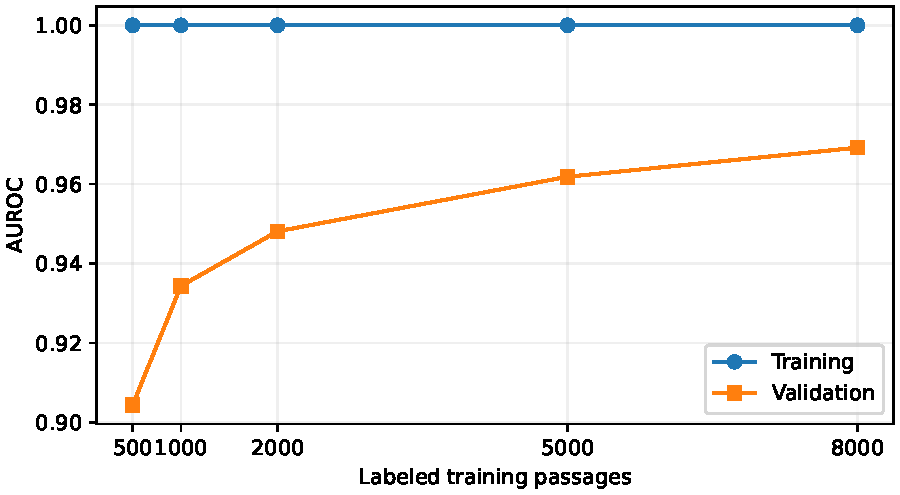
\includegraphics[width=0.85\linewidth]{figures/baseline_learning_curve.pdf}\end{center}
\question{Q2.3 [3 points].}{What does the curve suggest about overfitting, underfitting, and the value of more labeled examples?}
The model scores almost perfectly on the passages it learned from at every size, so it does not appear to be too simple for the training data. With only 500 passages, its validation AUROC is 0.9043; with 8000, it reaches 0.9690.

This large early gap between training and validation scores suggests overfitting: the model learns the small training sample better than it handles new passages. More labeled data helps, though the gains get smaller. The last 3000 passages raise validation AUROC by about 0.0065. Because we used one split and one sample at each size, we cannot predict how much another batch of labels would help.
\section{Learning from unlabeled data (5 points)}
\textbf{Learning goal:} test whether the additional 3,000 unlabeled passages help.
\question{Q3.1 [2 points].}{Describe one method that uses \texttt{unlabeled.csv} (e.g., self-training, confidence-based pseudo-labeling, clustering, or feature learning). How did you prevent validation-label leakage?}
We trained the character only logistic model (Model F) on 8000 labeled passages, and then used it to estimate AI probabilities for the unlabeled passages. We removed duplicate texts and any exact matches to labeled texts. We kept only confident predictions: $p\leq0.05$ became a provisional human label (540 passages), and $p\geq0.95$ became a provisional AI label (572 passages).

We trained a new copy of Model F on the original 8000 passages plus these 1112 provisionally labeled passages. We did not use validation labels to select or label them; those labels were used only to measure the result. The earlier v3 model used a different pseudo-labeling setup. The selected final ensemble turned semi-supervised training off, so this experiment does not measure a stage of the final submission.
\question{Q3.2 [2 points].}{Compare against a supervised baseline under the same held-out validation protocol.}
\begin{tabularx}{\linewidth}{@{}Yp{1.5in}@{}}\toprule Method & Validation AUROC \\ \midrule Supervised only (character baseline) & 0.968976 \\ With 1112 pseudo labeled rows & 0.968447 \\ \bottomrule\end{tabularx}
\question{Q3.3 [1 point].}{Did it help? Give a concrete, evidence-based explanation (including possible noise in pseudo-labels).}
Adding the 1112 provisionally labeled passages did not help Model F: validation AUROC fell from 0.968976 to 0.968447, a drop of 0.000529. A confident prediction can still be wrong, and retraining on wrong labels may repeat the first model's mistakes.

We do not know the true labels of those passages, so this is a possible explanation rather than a proven cause. We tried one data split and one pair of probability cutoffs; this result also does not tell us whether v3's different second stage helps.
\newpage
\section{Generalization and error analysis (20 points)}
\textbf{Learning goal:} characterize how well the selected model generalizes and where it fails. Use \textbf{labeled validation data}; hidden test labels and hidden domain/generator information are unavailable.

This section analyzes generalization using our fixed 2,000-row held-out validation partition (seed 42), which left 8,000 rows for training. Any features that learn from labels, including language models and reference genre statistics, used only the 8,000 training rows. We report performance for our 9-specialist base ensemble and examine the detailed subgroup and error breakdowns from the v3 pipeline that guided our final refinements.

\question{Q4.1 [5 points].}{Compare training and validation AUROC for your final selected model. Is there a gap? What explanations are plausible?}
For our final selected 9-specialist base ensemble, training AUROC was 1.000000 on the 8,000 training passages and held-out validation AUROC was 0.999449 on the 2,000 holdout passages. This represents a very small generalization gap of 0.000551 (compared with a gap of 0.000449 for the earlier v3 pipeline, which scored 1.0000 vs.\ 0.999551).

While this small gap shows that the ensemble fits the training distribution without collapsing on held-out text, the near-perfect validation score is still optimistic compared with the Kaggle test set. In the labeled training data, 66.0\% of AI passages contained a double newline compared with 0\% of human passages, allowing models to use formatting cues that appear less frequently or differently in test data. Furthermore, our test audit revealed that 14.4\% of test passages are poetry, a genre virtually absent from the training split (0.12\%). This test domain shift explains why our model scored 0.98629 (and 0.98640 after refinement) on Kaggle rather than 0.999.
\question{Q4.2 [5 points].}{Evaluate performance over at least three text-length bins (define the bins), or another observable subgroup available in your data. Explain why you chose the grouping.}
We grouped the v3 validation passages by word count to see whether length affects performance. Each of the three groups includes several hundred passages and both human and AI writing.

\begin{tabularx}{\linewidth}{@{}Yrr@{}}\toprule Subgroup / bin & Count & Validation AUROC \\ \midrule
75--165 words & 578 & 0.999661 \\
166--245 words & 832 & 0.999147 \\
246--350 words & 590 & 0.999942 \\
\bottomrule\end{tabularx}

The three groups contain 260/318, 481/351, and 259/331 human/AI passages  respectively. At a probability cutoff of 0.49, they have 4/2, 2/8, and 0/2 errors  respectively (human passages called AI / AI passages called human). Eight of the twelve AI passages wrongly classified as human are in the middle group. With so few errors, we cannot conclude that "medium length" passages are generally harder.
\question{Q4.3 [5 points].}{Analyze at least \textbf{five false positives and five false negatives} from your held-out validation set. Provide example IDs, predicted probabilities, and short failure hypotheses. Do not paste full passages unless essential.}
At the usual 0.50 probability cutoff, v3 wrongly flagged 4 human passages as AI (false positives) and missed 12 AI passages (false negatives). To examine at least five of each type, we lowered the cutoff to 0.49; this gives 6 false positives and 12 false negatives. The table shows five examples of each. The possible reasons come from a brief reading of the passages and are not proven causes.

\begin{tabularx}{\linewidth}{@{}p{0.64in}p{0.70in}p{0.98in}Y@{}}\toprule ID & Error type & P(AI) & Possible reason \\ \midrule
7767 & FP & 0.6644 & Its short and "polished" bio may read like an AI summary \\
4062 & FP & 0.5646 & The tidy and neat list of song facts may read like an AI summary as well \\
3660 & FP & 0.5634 & Repeated names and line breaks may look computer generated \\
5079 & FP & 0.5619 & The season recap repeats formal phrases which could look AI-written \\
3571 & FP & 0.4986 & Repeated opinions and the word \emph{movie} may look AI-written too \\
1362 & FN & 0.0535 & Dates and names may make this AI bio seem human written \\
9298 & FN & 0.1482 & Names and dated events may make this AI bio seem human written too \\
4519 & FN & 0.1503 & Lowercase first person wording may look like a casual human post \\
1834 & FN & 0.2234 & The timeline with dates may make this AI text seem like a human history article \\
5498 & FN & 0.2277 & Amounts and line breaks may make this AI text look like a human written recipe \\
\bottomrule\end{tabularx}

\smallnote{FP means human predicted AI; FN means AI predicted human (decision threshold 0.49). Auditing these specific failure types directly motivated the quote and verse refinements tested in Section 7.}
\question{Q4.4 [5 points].}{What recurring failure patterns did you identify, and how might you address one of them? Distinguish observed patterns from speculation.}
Among these 10 examples several human passages written like encyclopedia entries were labeled AI, while several AI biographies and one AI recipe were labeled human. An AI forum style passage was also missed, so genre alone does not explain every error.

We believe that ten examples are too few to tell us how common these problems are. We also saw evidence that formatting matters as well: the full first stage blend scored 0.999561 held out AUROC and its version without formatting features scored 0.987841.

We also want to note that the earlier v3 public Kaggle score was lower than its random-holdout score. A useful next test would reduce the weight of its formatting-based component and check passages from different genres and with altered line breaks. That could show whether the apparent formatting advantage survives a change in data; these v3 results alone do not tell us whether such a change would improve the final candidate's private score.
\newpage
\section{Open-ended improvements and insights (15 points)}
\textbf{Learning goal:} propose and test one improvement beyond the required baseline comparisons. This can be simple: a targeted feature change, alternate regularization scheme, ensemble, different representation, augmentation, or training approach. Sophistication alone does not earn credit.

\question{Q5.1 [3 points].}{What specific question or hypothesis motivated your improvement? What weakness or opportunity did you observe?}
A later version of our nine-model ensemble made 20 mistakes on a 2,000-passage holdout set: 6 false positives and 14 false negatives (evaluated separately from the v3 run in Section 6). Auditing these revealed that missed AI passages often began with Markdown quotes (\texttt{> }), human lists of names looked repetitive, and poetry suffered from verse line breaks. Our question was simple: Could targeted checks for these patterns improve the ensemble's predictions?


\question{Q5.2 [4 points].}{What exactly did you change? Describe the baseline, the new approach and what you held fixed for a fair comparison.}
Our baseline was our nine-model ensemble with fixed weights and predictions. Instead of retraining the whole pipeline, we added three automated checks inspired by our holdout autopsy: stripping leading Markdown quotes (\texttt{>}) to unmask technical abstracts, distinguishing capitalized proper-noun repetition from AI generation loops, and measuring syllable consistency and rhyme patterns in verse. To keep the comparison fair, the underlying ensemble was untouched; our code applied these checks programmatically across all 3,000 test passages without manual hand-labeling or external label retrieval.

\question{Q5.3 [4 points].}{What were the measured results?}
\begin{tabularx}{\linewidth}{@{}Yrrr@{}}\toprule
Step & Holdout AUROC & Errors at 0.50 & Kaggle public AUROC \\ \midrule
Original ensemble & 0.999449 & 20 & 0.98629 \\
Edits to known holdout errors & 0.999506 & 12 & --- \\
Exported test candidate & --- & --- & 0.98640 \\
\bottomrule\end{tabularx}

The holdout numbers come from the notebook's executed output. The public scores are recorded in the team's model results log. The holdout change is a post hoc diagnostic because the edited IDs were chosen after their errors were known; the Kaggle score measures a separate test-file candidate.

\question{Q5.4 [4 points].}{What did you learn? Did the results support the hypothesis? What limits the conclusion, and what would you try next?}
Targeted adjustments improved public AUROC from 0.98629 to 0.98640, supporting our hypothesis. We learned that n-gram models can over-index on structural cues---flagging classic poetry as AI due to verse line breaks, or missing AI text masked by quotes. The primary limitation is threshold brittleness (e.g., rhyme $> 0.4$ could misrank an unseen tight-meter human poem), and the holdout error drop (20 to 12) was a post hoc diagnostic. Next, we would avoid post-hoc edits by feeding rhyme, meter, and unmasked text directly into the Stage-1 feature matrix for native tree training.

\newpage
\enlargethispage{5\baselineskip}
\section{Code submission, reproducibility and AI assistance (10 points)}
\textbf{Submission format:} Submit a \textbf{GitHub PR URL} against the course repository. We will inspect the final code and its development history, not just the final snapshot. Do not squash away meaningful intermediate commits before review. Template \href{https://github.com/sekhari/human-or-ai-submissions}{here}.

\question{Q6.1 [5 points].}{Provide the PR URL, the entrypoint for training/evaluation, and the command used to generate \texttt{submission.csv}. State dependencies and random seeds.}
Our GitHub PR URL is \href{https://github.com/sekhari/human-or-ai-submissions/pull/6}{PR Link}. To reproduce the final CSV, use Python 3.12 on CPU and place \texttt{train.csv}, \texttt{unlabeled.csv}, \texttt{test.csv}, and \texttt{sample\_submission.csv} in the repository's \texttt{data/} directory. From the repository root, run:
\begin{quote}\vspace{-0.5em}\footnotesize\ttfamily
python -m pip install -r submissions/team-35/requirements.txt nbconvert ipykernel\\
cd submissions/team-35\\
jupyter nbconvert --to notebook --execute --inplace final\_model\_improvements.ipynb\\
jupyter nbconvert --to notebook --execute --inplace error\_directed\_model\_refinement.ipynb\\
cp submission\_error\_directed\_refinement.csv submission.csv
\vspace{-0.5em}\end{quote}
The first notebook generates base ensemble predictions and cached artifacts; the second executes targeted quote and verse calibrations to produce \texttt{submission.csv}. Seed 42 is pinned across all models (seed 43 for secondary checks). Data and generated CSVs remain outside Git.

\question{Q6.2 [3 points].}{Give two or three examples of changes you made during development. Link to relevant commits or PR discussion and briefly explain what the experiments taught you.}
\begin{itemize}[topsep=0pt,itemsep=0pt,parsep=0pt]
\item \href{https://github.com/jaminatore/human-or-ai-submissions/commit/5e8256c}{\texttt{5e8256c}}: We measured a character-pattern baseline at several training sizes. More labeled passages improved validation AUROC, while adding confident pseudo-labels did not help in that separate test.
\item \href{https://github.com/jaminatore/human-or-ai-submissions/commit/8930188}{\texttt{8930188}}: We expanded the ensemble and checked that training did not use held-out labels. The public score improved, but the test gap remained.
\item \href{https://github.com/jaminatore/human-or-ai-submissions/commit/c7f2ca6}{\texttt{c7f2ca6}}: Quote and verse adjustments reached 0.98640 publicly. The ID-edited holdout comparison was only diagnostic.
\end{itemize}

\question{Q6.3 [2 points].}{How did you use AI tools (such as Claude, ChatGPT or Copilot) for code, debugging, analysis or writing? What did you verify or modify yourself?}
We used AI assistants, including ChatGPT/Codex, to brainstorm approaches, draft code, suggest improvements, and help format and organize files and report text. The team chose the direction of the experiments, reviewed and changed suggested code and wording, checked the reasoning, and validated the reported results. We compared numerical claims with saved notebook outputs and Kaggle score records rather than treating AI suggestions as measurements.

\vspace{-0.3em}
\textbf{AI policy.} You may use AI assistants for coding, debugging, explanations, brainstorming, and editing. We expect each team to exercise its own judgment, run experiments, check outputs, and understand its submitted approach. Sending the entire assignment to an AI tool and submitting its unverified output without meaningful involvement does not satisfy the objectives of this project. We will use the PR history, reproducible experiments and report together as evidence of engagement. \emph{Commit counts and the presence of AI-generated code are not themselves grading criteria.} Do not fabricate results or retrieve hidden test labels.

\vspace{-0.4em}
\section*{Final submission checklist}
\vspace{-0.2em}
\begin{itemize}[label=$\boxtimes$,topsep=0pt,itemsep=0pt,parsep=0pt]
\item Final probabilities submitted to Kaggle for every \texttt{test.csv} ID.
\item Completed report, with all required answers, tables, figures and sources, submitted as PDF.
\item GitHub PR linked on the report title page and in the course submission portal.
\item Code and dependencies recreate final predictions (within reasonable numerical tolerance).
\item Relevant experiments and seed/configuration details are recorded.
\item AI-use disclosure is complete; hidden labels were not retrieved externally.
\end{itemize}

\end{document}
